\chapter{Análise e Resultados} \label{analiseResultados}
Este capítulo visa apresentar os seguintes itens: "Critérios de Análise", "Análise"\ e "Resultados".

Para realização da análise proposta nesse trabalho, utilizaremos uma série de elementos que constituirão a metodologia de comparação entre as soluções que apresentem documentações públicas disponíveis e com informação necessária e suficiente.

\section{Critérios de Análise}

Com base nos conceitos apresentados por \citeonline[p.305]{wazlawick2012}, que define os atributos de qualidade internos, externos e de uso de produtos de software; e pela autora \citeonline{wangenheim2017}, que define heurísticas para assegurar que os produtos são usáveis, esta seção tem por objetivo apresentar os critérios que devem ser considerados na avaliação das soluções para busca de dados musicais, de modo a compará-las e facilitar a escolha pela mais apropriada para uma determinada situação.

Neste trabalho foi criado um conjunto de heurísticas para permitir uma boa análise da eficiência e adequação funcional das soluções apresentadas, sendo utilizado informações disponibilizadas nas documentações próprias de cada solução comercial e acadêmica.

Para a análise da usabilidade será feito uma adaptação do MATcH Checklist disponibilizado pelo Grupo de Qualidade de Software (GQS) da UFSC, onde o conjunto de perguntas possui uma escala de resposta com 3 opções: Sim (o app atende o objetivo), Não (o app não atende o objetivo) e Não se aplica (a questão avaliada não se aplica).

Assim sendo, os seguintes critérios e subcritérios são considerados:

\begin{itemize}
    \item Eficiência de desempenho: Trata-se da otimização do uso de recursos de tempo e espaço. Espera-se que o sistema seja o mais eficiente possível de acordo com o tipo de problema que ele soluciona:
    \begin{itemize}
        \item \textit{Comportamento em relação ao tempo}: Este critério mede o tempo que o sistema leva para processar suas funções, ou seja, o tempo de reconhecimento/busca de uma música;
        \item \textit{Utilização de recursos}: Avalia a complexidade das estratégias e algoritmos utilizados na recuperação de informação musical;
        \item \textit{Bitrate}: Este critério mede a qualidade do áudio. Essa qualidade consiste no número médio de bits que será comprimido em um segundo de dados. A unidade utilizada é o KBPS ou 1000 BITS por segundo.
    \end{itemize}
    \item Adequação Funcional: A adequação funcional mede o grau em que o produto oferece funções que satisfazem necessidades estabelecidas e implicadas quando o produto é usado sob condições especificadas:
    \begin{itemize}
        \item \textit{Disponibilidade}: Avalia a disponibilidade da aplicação em diferentes plataformas;
        \item \textit{Modelo de desenvolvimento}: Avalia se a aplicação é de código aberto, dando a possibilidade para que qualquer um consulte, examine ou modifique o produto.
        \item \textit{Integrações}: Avalia se permite extensões e/ou integrações com outras aplicações;
        \item \textit{Acessibilidade}: Avalia se a aplicação possui acesso ao acervo de músicas online e/ou offline;
        \item \textit{Busca de dados}: Avalia se a aplicação foi projetada para \textit{matching} exato ou aproximado;
        \item \textit{Inclusão da dados}: Avalia se a aplicação permite o envio de músicas feito pelo usuário;
        \item \textit{Modelo de pagamento}: Avalia o custo da aplicação, como por exemplo: Gratuito, Pago ou Freemium.
    \end{itemize}
    \item Usabilidade: Avalia o grau no qual o produto tem atributos que permitem que seja entendido, aprendido, usado e que seja atraente ao usuário, quando usado sob condições especificadas:
    \begin{itemize}
        \item \textit{Visibilidade do status do sistema}: O sistema deve sempre manter o usuário informado sobre o que está acontecendo, por exemplo, os componentes interativos selecionados são claramente distintos dos demais?
        \item \textit{Prevenção de erros}: Mensagens de erros devem ser claras e objetivas, devem indicar o problema com precisão e sugerir uma solução;
        \item \textit{Flexibilidade e eficiência de uso}: Permitir configuração de ações frequentes, por exemplo, as funções mais utilizadas são facilmente acessadas?
        \item \textit{Estética e Design minimalista}: Mensagens de diálogos não devem conter informações irrelevantes, por exemplo, o menu é esteticamente simples e claro, com opções fáceis de encontrar, dispostas em uma ordem lógica e com títulos curtos?
        \item \textit{Pouca interação homem/dispositivo}: Qualquer informação deve ser fácil de pesquisar e deve ser focada na tarefa do usuário, por exemplo, a navegação da solução é intuitiva, é fácil chegar à tela desejada?
    \end{itemize}
\end{itemize}

\section{Análise}

À partir da Tabela \ref{comparacaoCriterios}, podemos verificar que dentre as opções escolhidas para as soluções comerciais, em sua grande maioria o modelo de desenvolvimento é fechado, ou seja, seu código não pode ser alterado, mas possuem Web APIs disponibilizadas para a comunidade de desenvolvedores, para que a solução possa ser incorporada a seus próprios sites e aplicações.

Das 9 soluções analisadas, 5 possuem reconhecimento de músicas de forma aproximada, ou seja, que é possível realizar buscas de músicas através da voz, seja cantando ou cantarolando. E 4 soluções com o reconhecimento de músicas de forma exata, onde é necessário uma parte de áudio "original"\ e/ou por conteúdo, que seriam as buscas através de cadeias de caracteres.

Apenas 3 soluções permitem a inclusão de músicas criadas por usuários, porquanto as outras 6 apenas permitem a inclusão de novas músicas através de contatos com gravadoras e/ou artistas. Destas 3, duas reconhecem músicas de forma aproximada, ACRCloud e Musipedia. A primeira é um serviço de nuvem, até o momento, o maior banco de dados de músicas, sendo também um serviço utilizado pela maioria das outras soluções aqui analisadas, como MusiXmatch e Deezer, onde fornece o mecanismo de reconhecimento das músicas através do método de Fingerprint.

Musipedia é uma wikipedia de músicas, que aceita contribuições musicais de diversas formas: através da voz, partes de músicas, ou até em formato MIDI (quando o som é criado digitalmente). Não foi encontrado documentação que especificasse o método ou algoritimo utilizado para o reconhecimento das músicas, mas podemos dizer que possivelmente também utiliza o método de Fingerprint.

Com isso, é possível verificar que as soluções com o reconhecimento de músicas de forma aproximada e as soluções com o reconhecimento de forma exata utilizam o mesmo método de Fingerprint. E apesar de utilizarem o mesmo método, a forma como pode ter sido desenvolvido é o que gerou a vantagem competitiva dentre os concorrentes do mesmo ramo.

Em especial temos o SoundHound, que utiliza da tecnologia de Inteligência Artificial (IA) \abreviatura{IA}{Inteligência Artificial} para o reconhecimento das músicas. É possível realizar buscas através da voz, cantarolando, batucando ou até mesmo uma parte de áudio "original". Conforme os usuários cantam em busca de uma música e conforme a escolha da música do resultado amostrado, a IA associa a cantoria para aquela música. Então, quanto mais cantar e buscar as músicas "certas"\ para a cantoria, a taxa de acerto aumenta, e assim vai se formando uma rede totalmente interligada para o reconhecimento correto das músicas.

Há também as soluções que utilizam o método de Recuperação por Conteúdo, que seriam as cadeias de caracteres, em busca do título, do álbum ou do gênero da música - os que chamamos de metadados, conforme já foi explícitado em seções anteriores deste trabalho. Destas soluções podemos citar o Spotify e o SoundCloud.

O Spotify é um aplicativo multiplataforma, a solução que faz sucesso dentre os usuários. A busca das músicas é feita exclusivamente através de texto, não é possível adicionar músicas criadas pelo usuário, mas é possível criar playlists com as suas músicas preferidas, além de poder ouvi-las off-line - um recurso oferecido por poucos, apenas 3 das 9 analisadas.

O seu sistema de busca é dividido em 3 partes: cache, peer-to-peer\footnote{(do inglês par-a-par ou simplesmente ponto-a-ponto, com sigla P2P) é uma arquitetura de redes de computadores onde cada um dos pontos ou nós da rede funciona tanto como cliente quanto como servidor, permitindo compartilhamentos de serviços e dados sem a necessidade de um servidor central.} e servidor. Ao escutar uma música através do smartphone, o sistema irá primeiro verificar se a música já se encontra baixada na memória cache para agilizar o processo, em caso negativo é feita a conexão diretamente com o servidor do Spotify, ao mesmo tempo que o método busca "peers"\ entre milhões de usuários para que a música que se queira ouvir, seja baixada o mais rápido possível. Veja a Figura \ref{fig:spotifyp2p}.

\begin{figure}[!htb]
   \centering
   \caption{Sistema de Busca do Spotify}\label{fig:spotifyp2p} 
   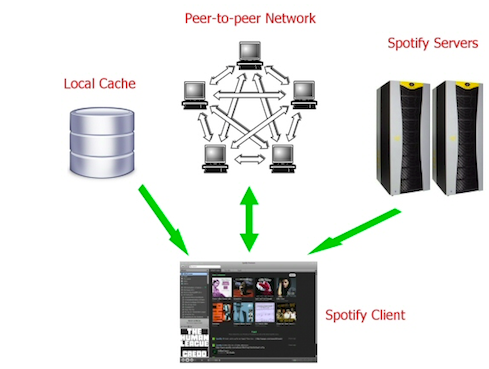
\includegraphics[scale=0.8]{figuras/spotifyp2p.png}
   \\Fonte: \cite{kreitz2010}
\end{figure}

Nas três divisões, em um dado momento, a comparação de strings será feita para verificar se a palavra buscada se encontra entre os metadados armazenados nos arquivos de áudio. Da mesma forma ocorre para a comparação de strings feita no SoundCloud.

Em relação ao tempo, as diferenças foram constatadas verificando o tipo de método utilizado para o reconhecimento/busca de músicas. Para as soluções utilizando a Recuperação por Conteúdo poderiam demorar até 30s, dependendo da conexão de Internet, para o retorno da amostra de resultados. Já as soluções utilizando Fingerprint, varia de 8s até 13s e utilizando IA até 5s. Uma análise feita apenas sobre o comportamento da solução em relação ao tempo não seria relevante, já que entre 30s e 5s é relativo a situação em que você estará no momento.

Com excessão do ACRCloud, todas possuem versões gratuitas para uso, com a versatibilidade de poder escolher pagar uma mensalidade e não ter interrupções e propagandas entre as músicas. E apenas as soluções de reconhecimento de músicas possuem inegrações com outros serviços e/ou aplicações.

Com o Shazam, por exemplo, é possível integrar ao Spotify e então ao encontrar uma música, poder ouvi-la por completo. Da mesma forma para o SoundHound, além de ser possível o compartilhamento da sua pesquisa com o Twitter. 

Com o MusiXmatch, por exemplo, integrado com o Spotify, ao encontrar uma música, você acompanha a música com a letra em tempo real. Já o ACRCloud, como um serviço de reconhecimento de músicas, possui o maior número de integrações, mas sendo utilizado no desenvolvimento em conjunto com a aplicação principal, pois sua disponibilidade atual é apenas via Web.

De forma mais individual quanto a usabilidade, cada solução tem a sua particularidade, que atrai ou afasta o usuário.

O MusicID (Ver Figura \ref{fig:musicID}) é extremamente simples, navegação intuitiva, sem muitas funcionalidades e de fácil execução, o uso é exclusivo para o reconhecimento de músicas. Os componentes interativos são claramente distintos dos demais, com ícones compreensíveis, intuitivos e possui uma linguagem clara e concisa. Funciona corretamente, sem apresentar problemas. O menu é esteticamente simples, claro e sem propagandas. Da mesma forma para o Shazam (Ver Figura \ref{fig:shazam}), extremamente simples, com o diferencial de tirar fotos de QRCodes para fazer a busca da música.

\begin{figure}[!htb]
   \centering
   \caption{MusicID}\label{fig:musicID} 
   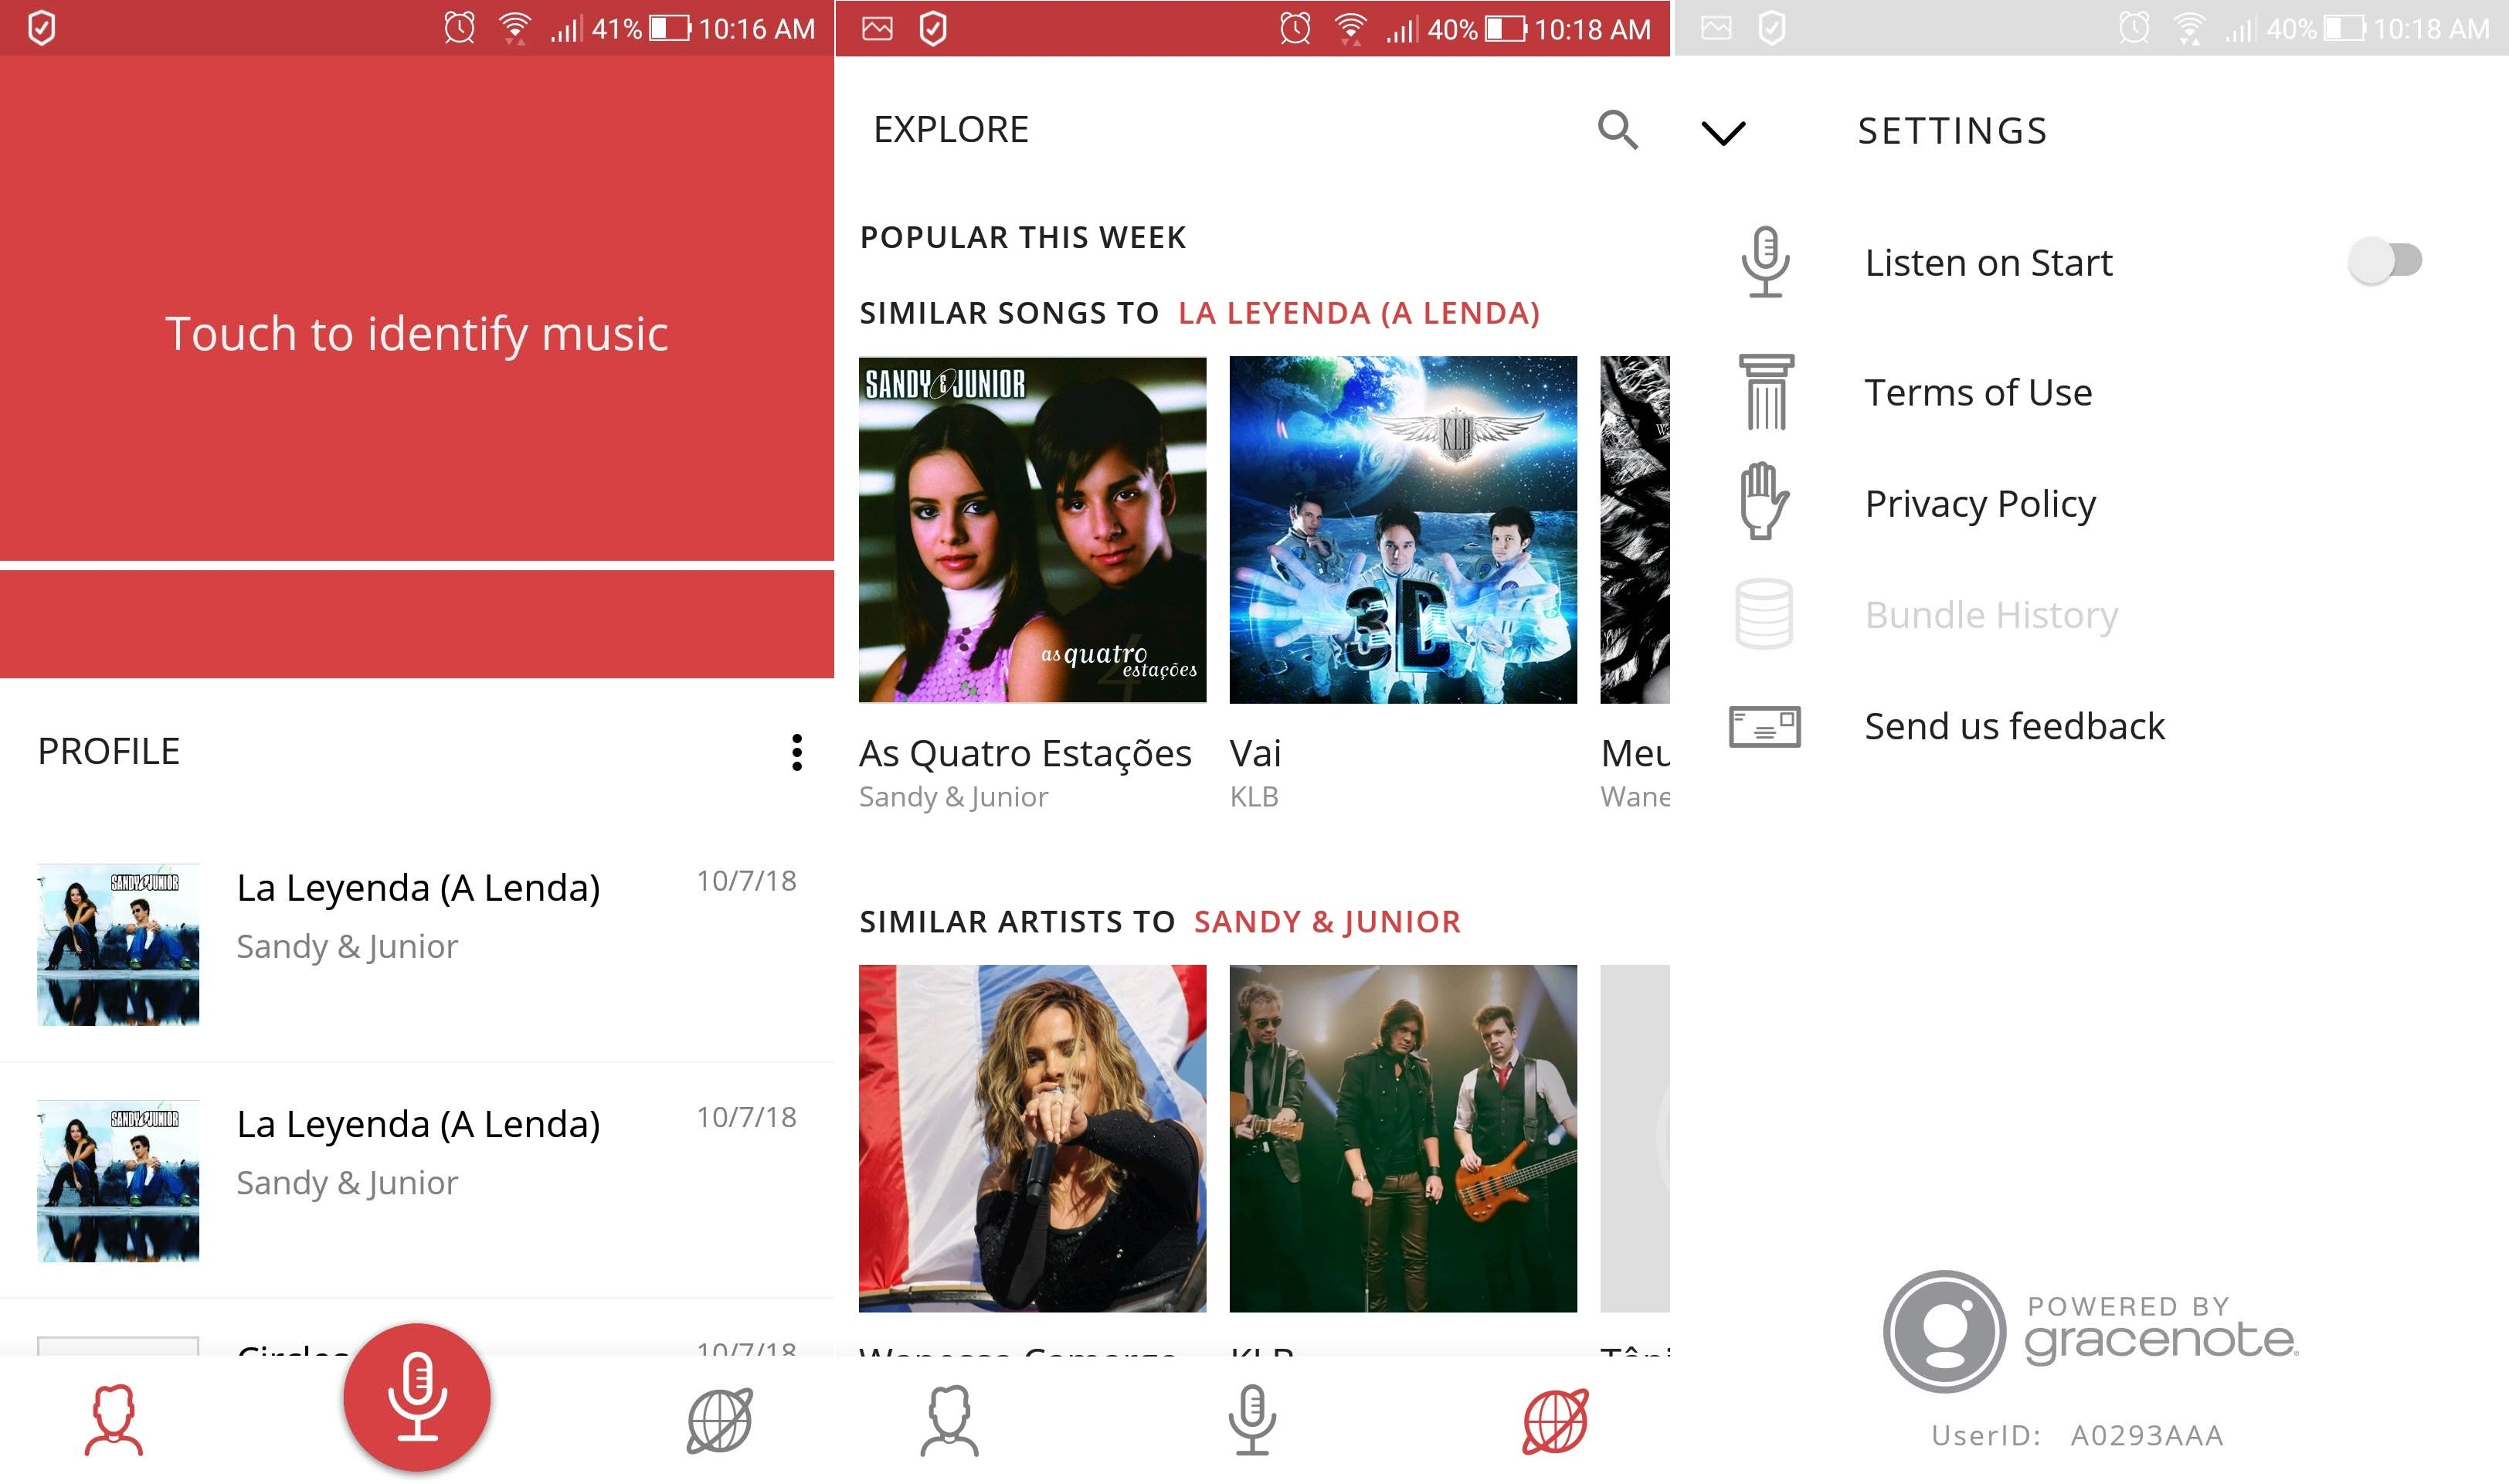
\includegraphics[scale=0.17]{figuras/MusicID.jpg}
   \\Fonte: Elaborado pela autora
\end{figure}

\begin{figure}[!htb]
   \centering
   \caption{Shazam}\label{fig:shazam} 
   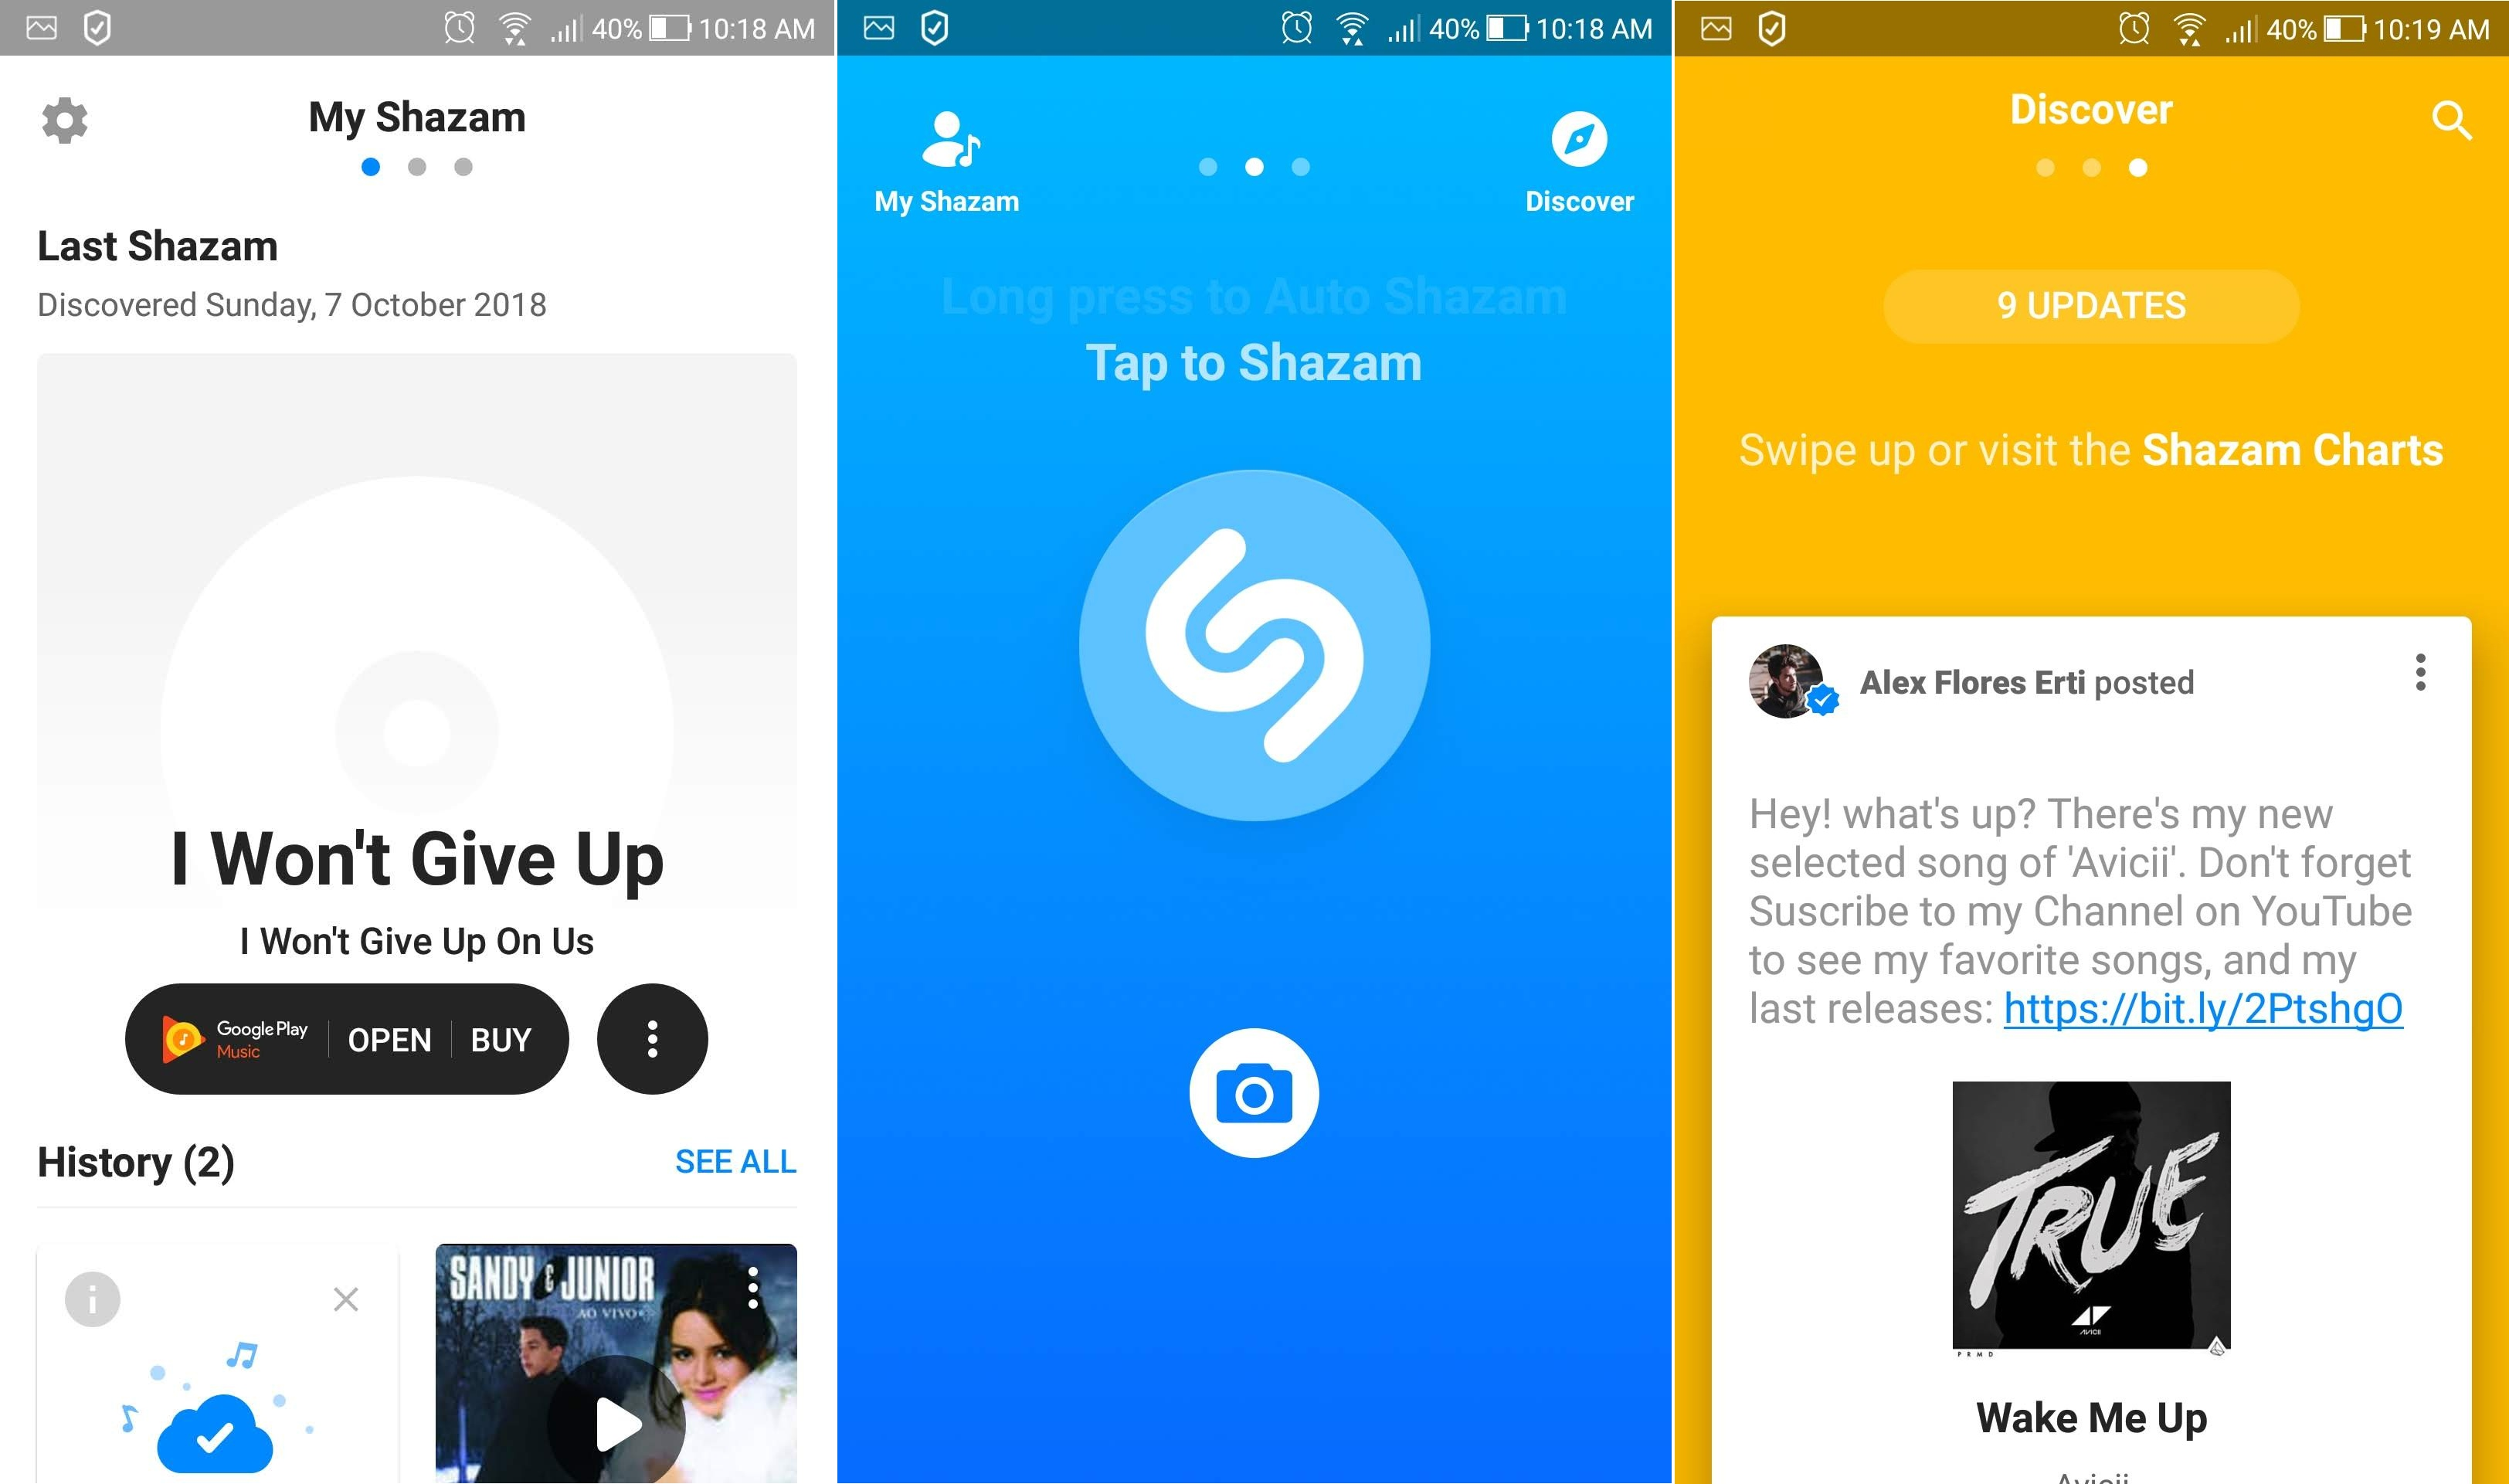
\includegraphics[scale=0.17]{figuras/shazam.jpg}
   \\Fonte: Elaborado pela autora
\end{figure}

O SoundHound (Ver Figura \ref{fig:soundHound}) é de fácil execução, possui mais funcionalidades além do reconhecimento de músicas, como a possibilidade de criar playlists e o compartilhamento com o Twitter. Além das informações básicas sobre a música, o aplicativo sugere alguns vídeos que podem ser assistidos diretamente no SoundHound. Os componentes interativos são claramente distintos dos demais, com ícones compreensíveis, intuitivos, linguagem clara e de textos curtos. Funciona corretamente, sem apresentar problemas. O menu é esteticamente simples, mas possui propagandas, o que polui a tela e adquirindo a versão paga as propagandas são retiradas.

\begin{figure}[!htb]
   \centering
   \caption{SoundHound}\label{fig:soundHound} 
   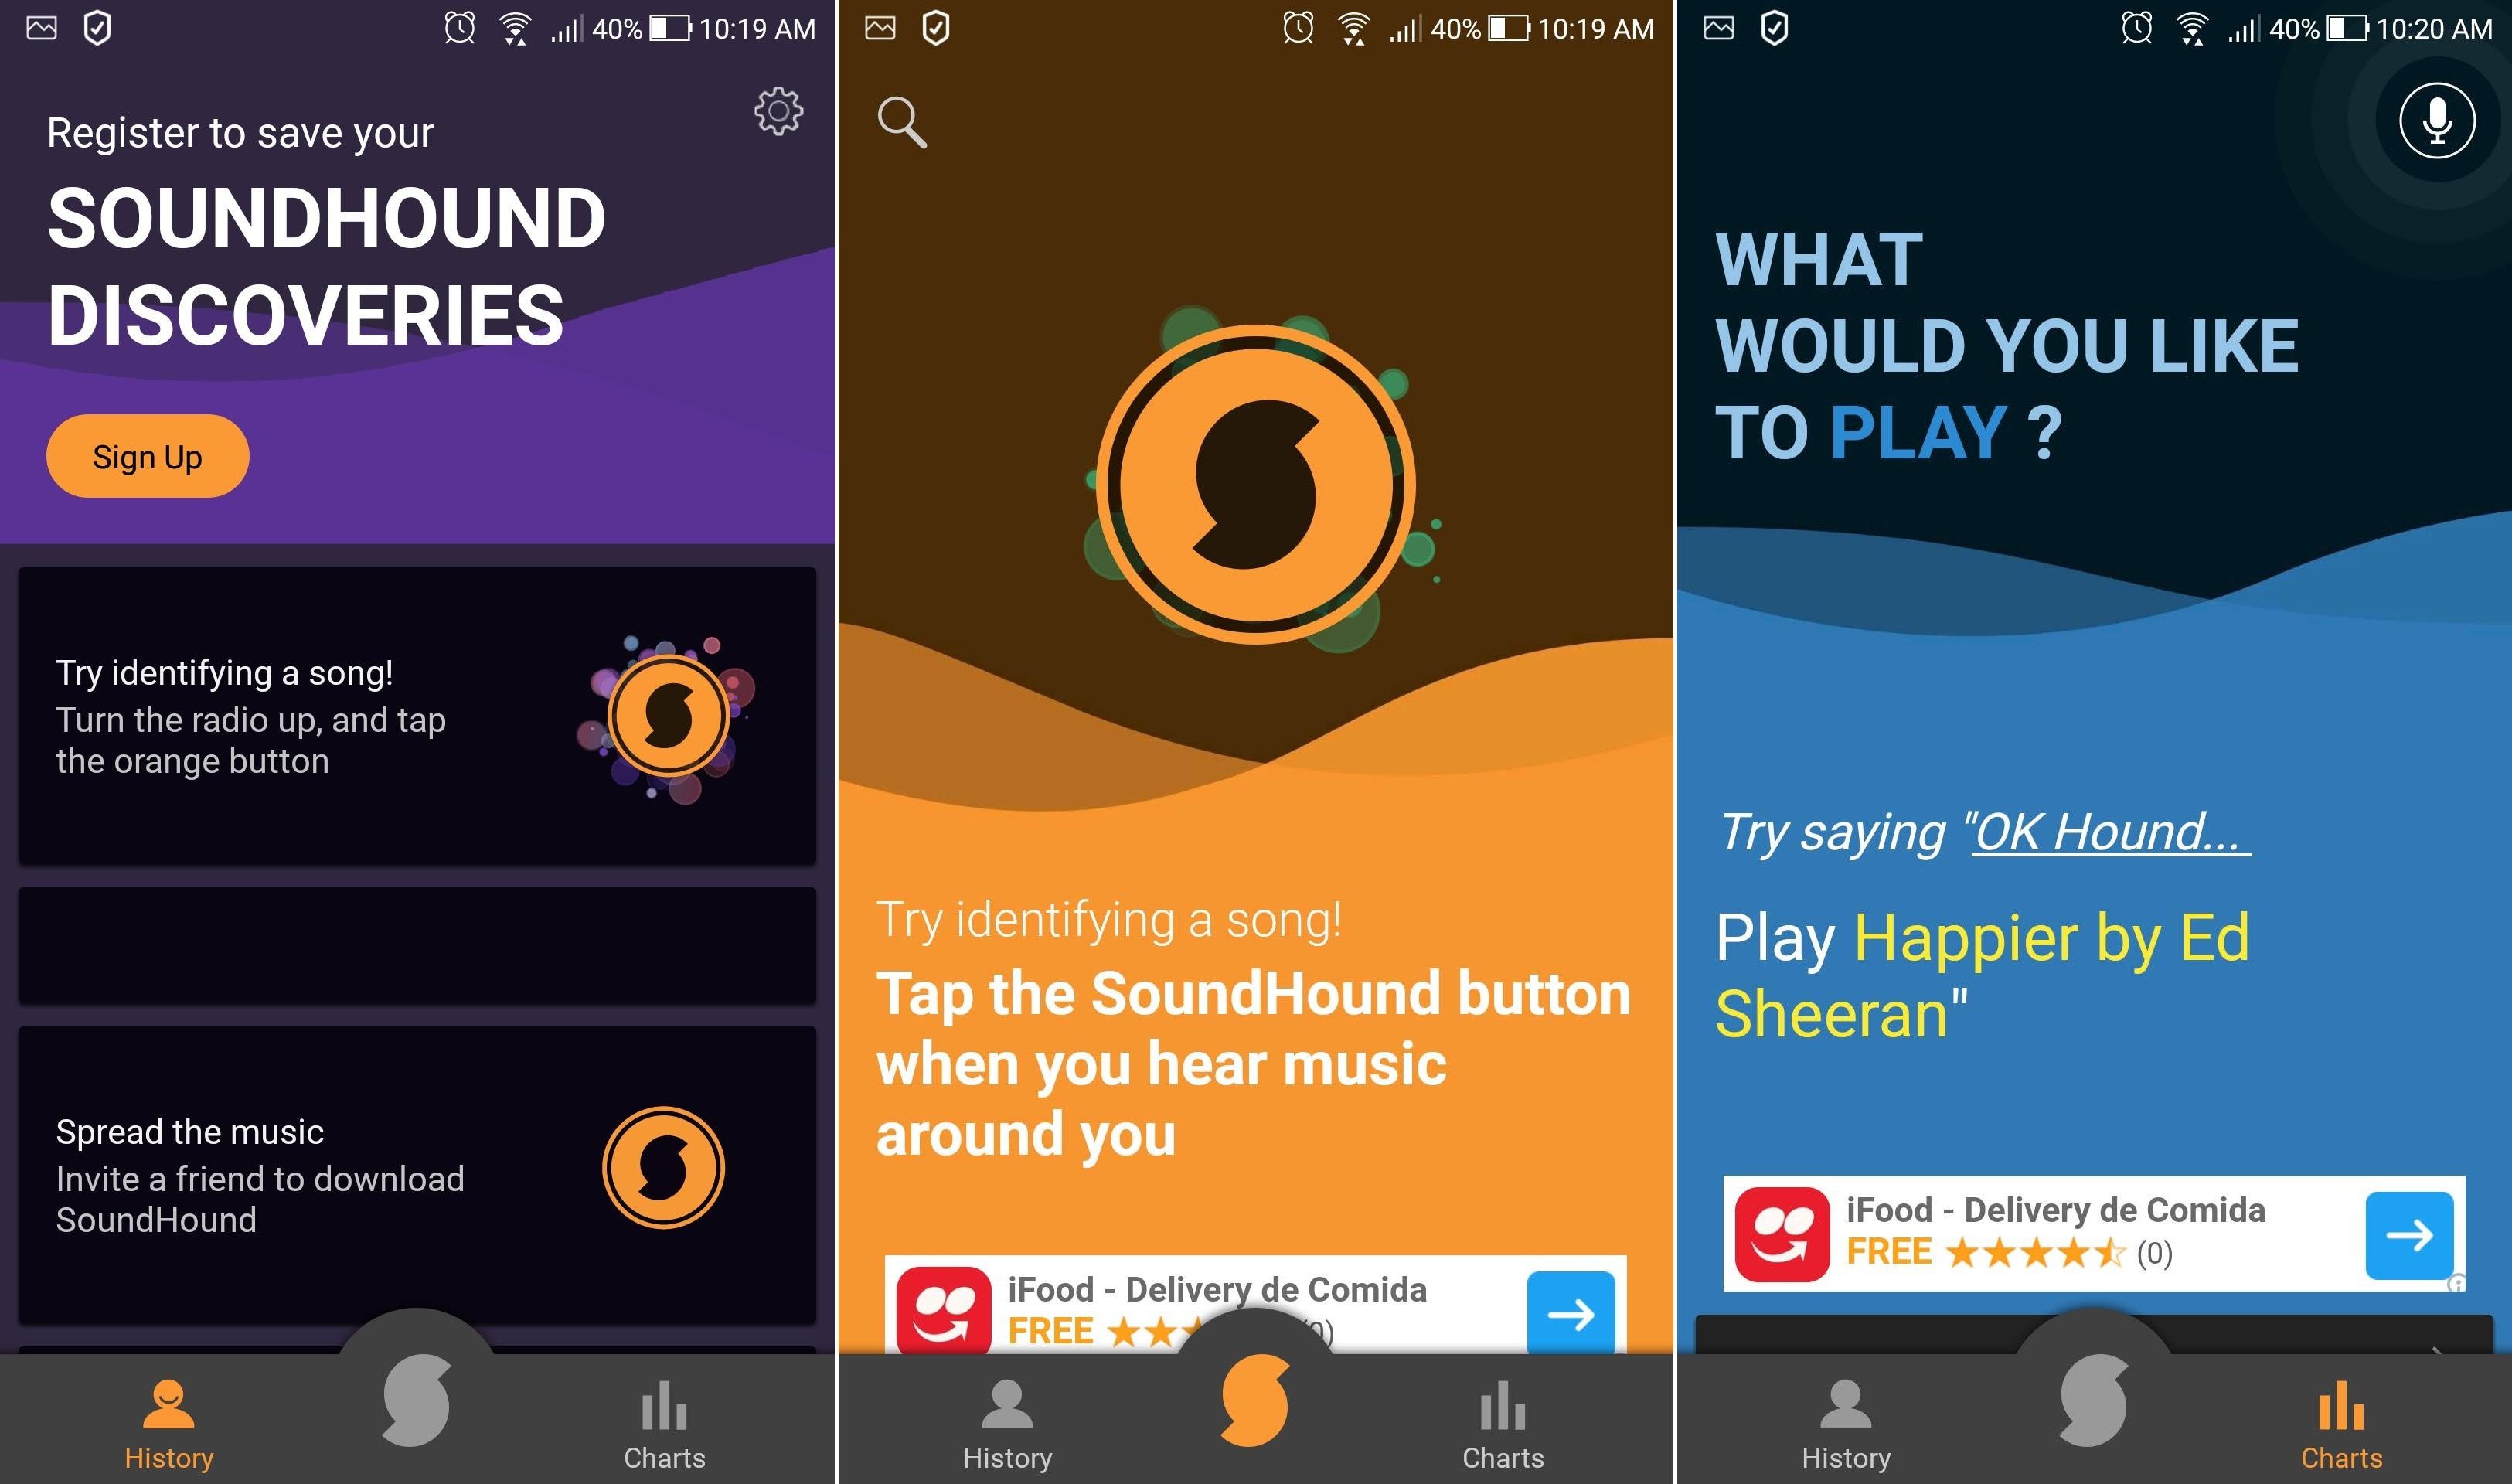
\includegraphics[scale=0.17]{figuras/soundhound.jpg}
   \\Fonte: Elaborado pela autora
\end{figure}

O Deezer (Ver Figura \ref{fig:deezer}) é simples, navegação intuitiva, sua busca por músicas era inicialmente por metadados, ou seja, a digitação do título, álbum ou genero da música. Além da criação de playlists, hoje possui também a funcionalidade de reconhecimento de músicas e a possibilidade do download das músicas para uso offline. Os componentes interativos são claramente distintos dos demais, com ícones compreensíveis, intuitivos, linguagem clara e de textos curtos. Funciona corretamente, sem apresentar problemas. O menu é esteticamente simples, mas em sua versão gratuita possui propagandas, o que polui a tela e apenas adquirindo a versão paga as propagandas são retiradas.

\begin{figure}[!htb]
   \centering
   \caption{Deezer}\label{fig:deezer} 
   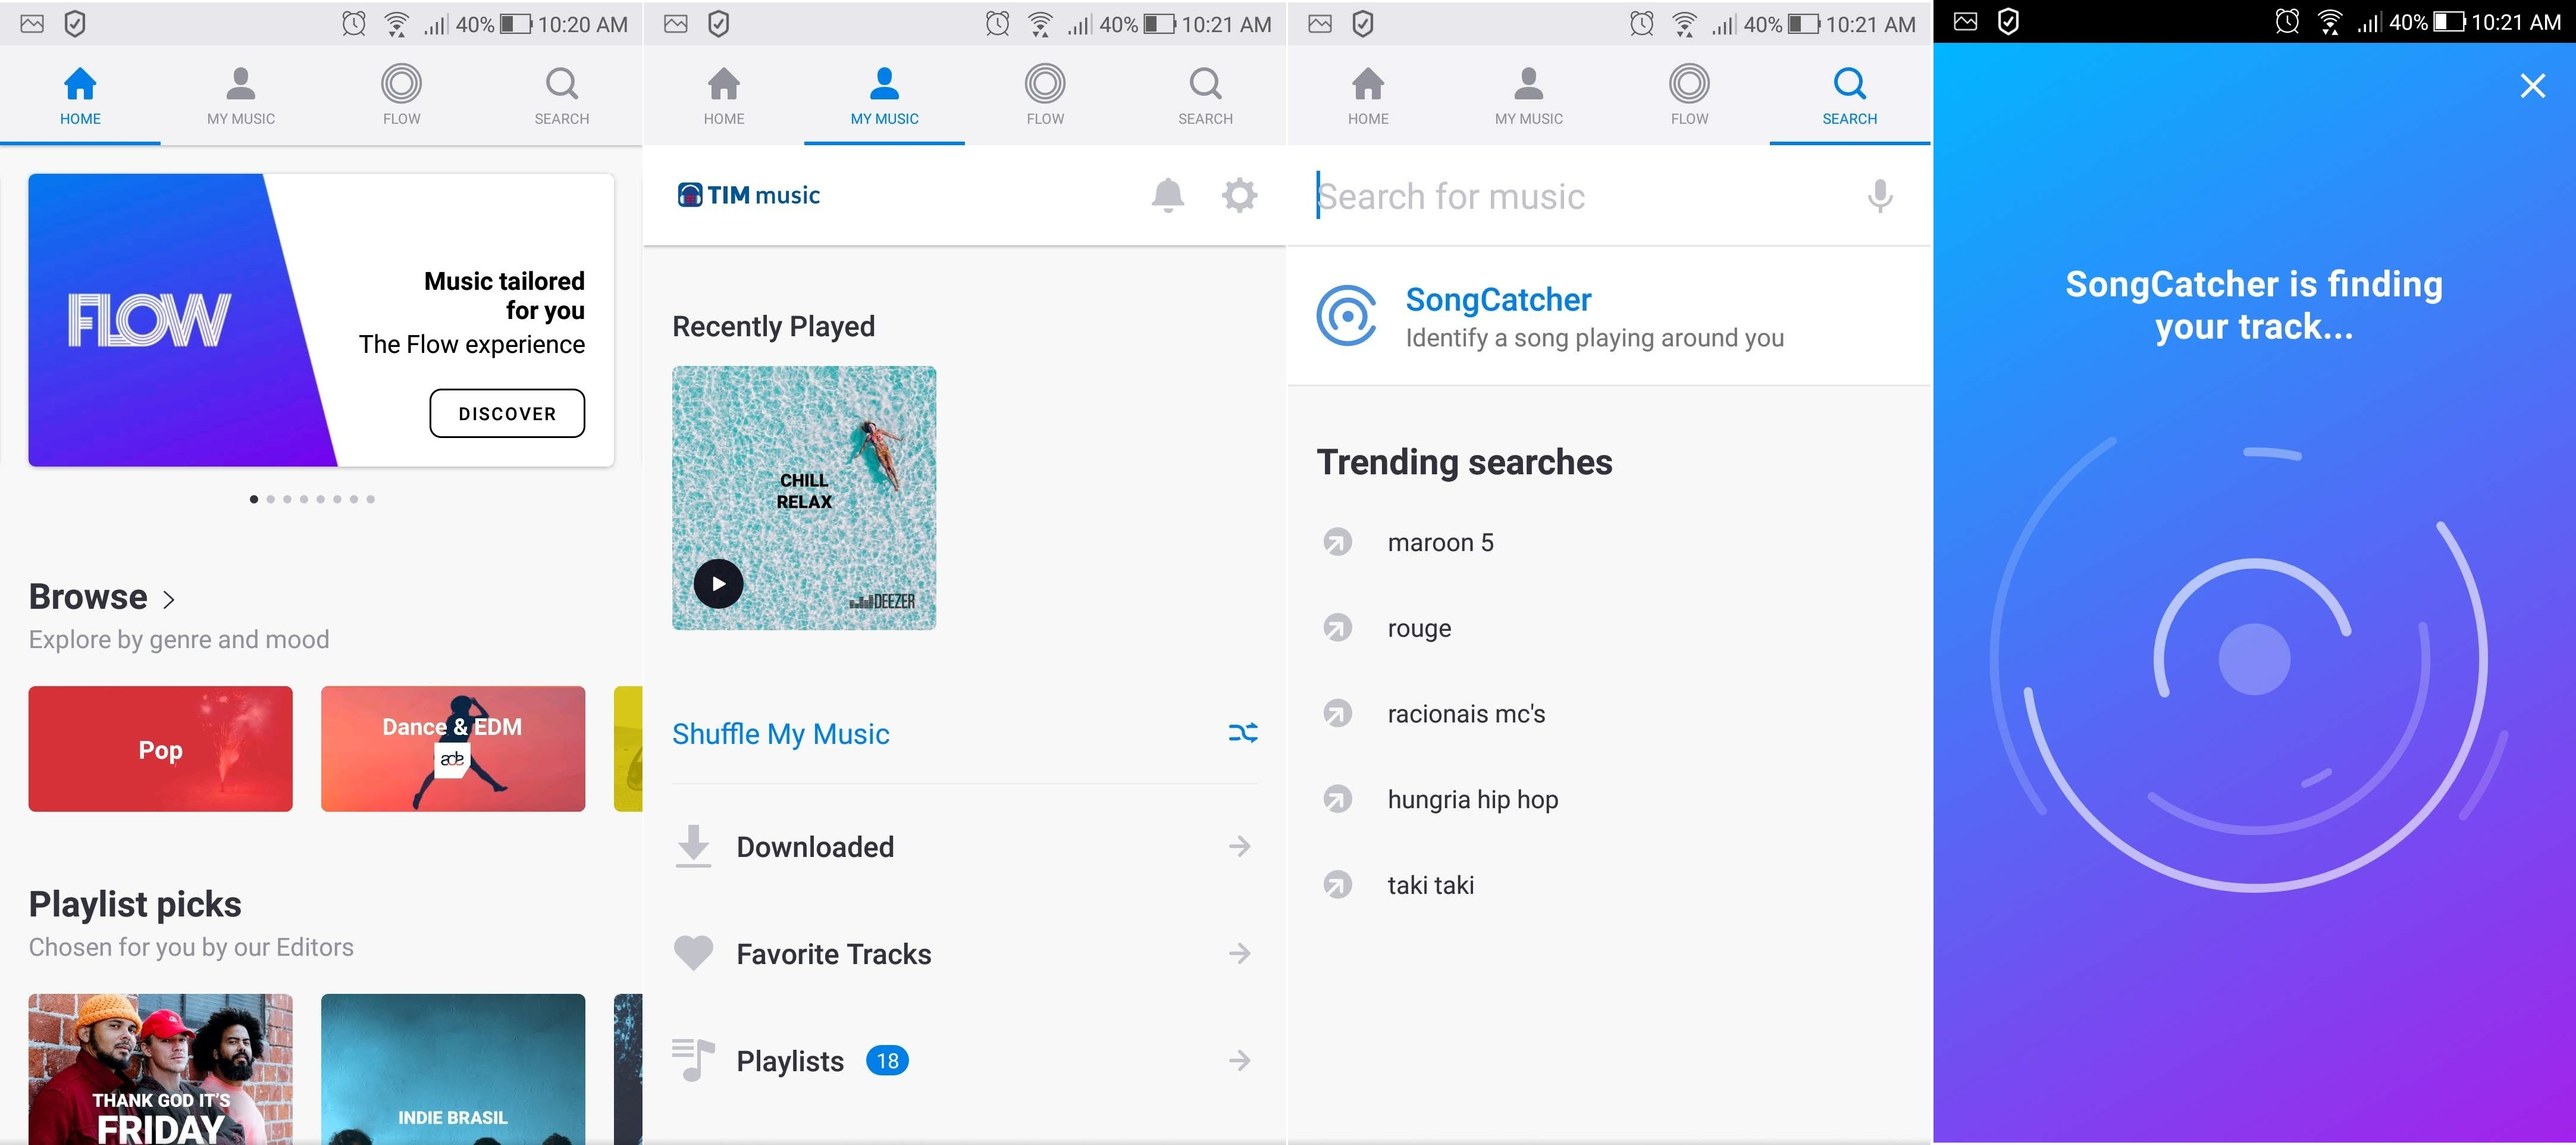
\includegraphics[scale=0.13]{figuras/deezer.jpg}
   \\Fonte: Elaborado pela autora
\end{figure}

O Spotify (Ver Figura \ref{fig:spotify}) é bem similar ao Deezer em questão de funcionalidades, a diferença é que o Spotify não possui funcionalidade para o reconhecimento das músicas, utilizando a busca por música exclusivamente por metadados. Os componentes interativos são claramente distintos dos demais, com ícones compreensíveis, intuitivos, linguagem clara e de textos curtos. Funciona corretamente, sem apresentar problemas. O menu é esteticamente simples, sua versão gratuita conta com propaganda entre as músicas, o que é bem irritante e acaba forçando o usuário a obter uma versão premium para, desta forma, usufruir de todas as possibilidades do aplicativo, como o download de músicas para uso offline.

\begin{figure}[!htb]
   \centering
   \caption{Spotify}\label{fig:spotify} 
   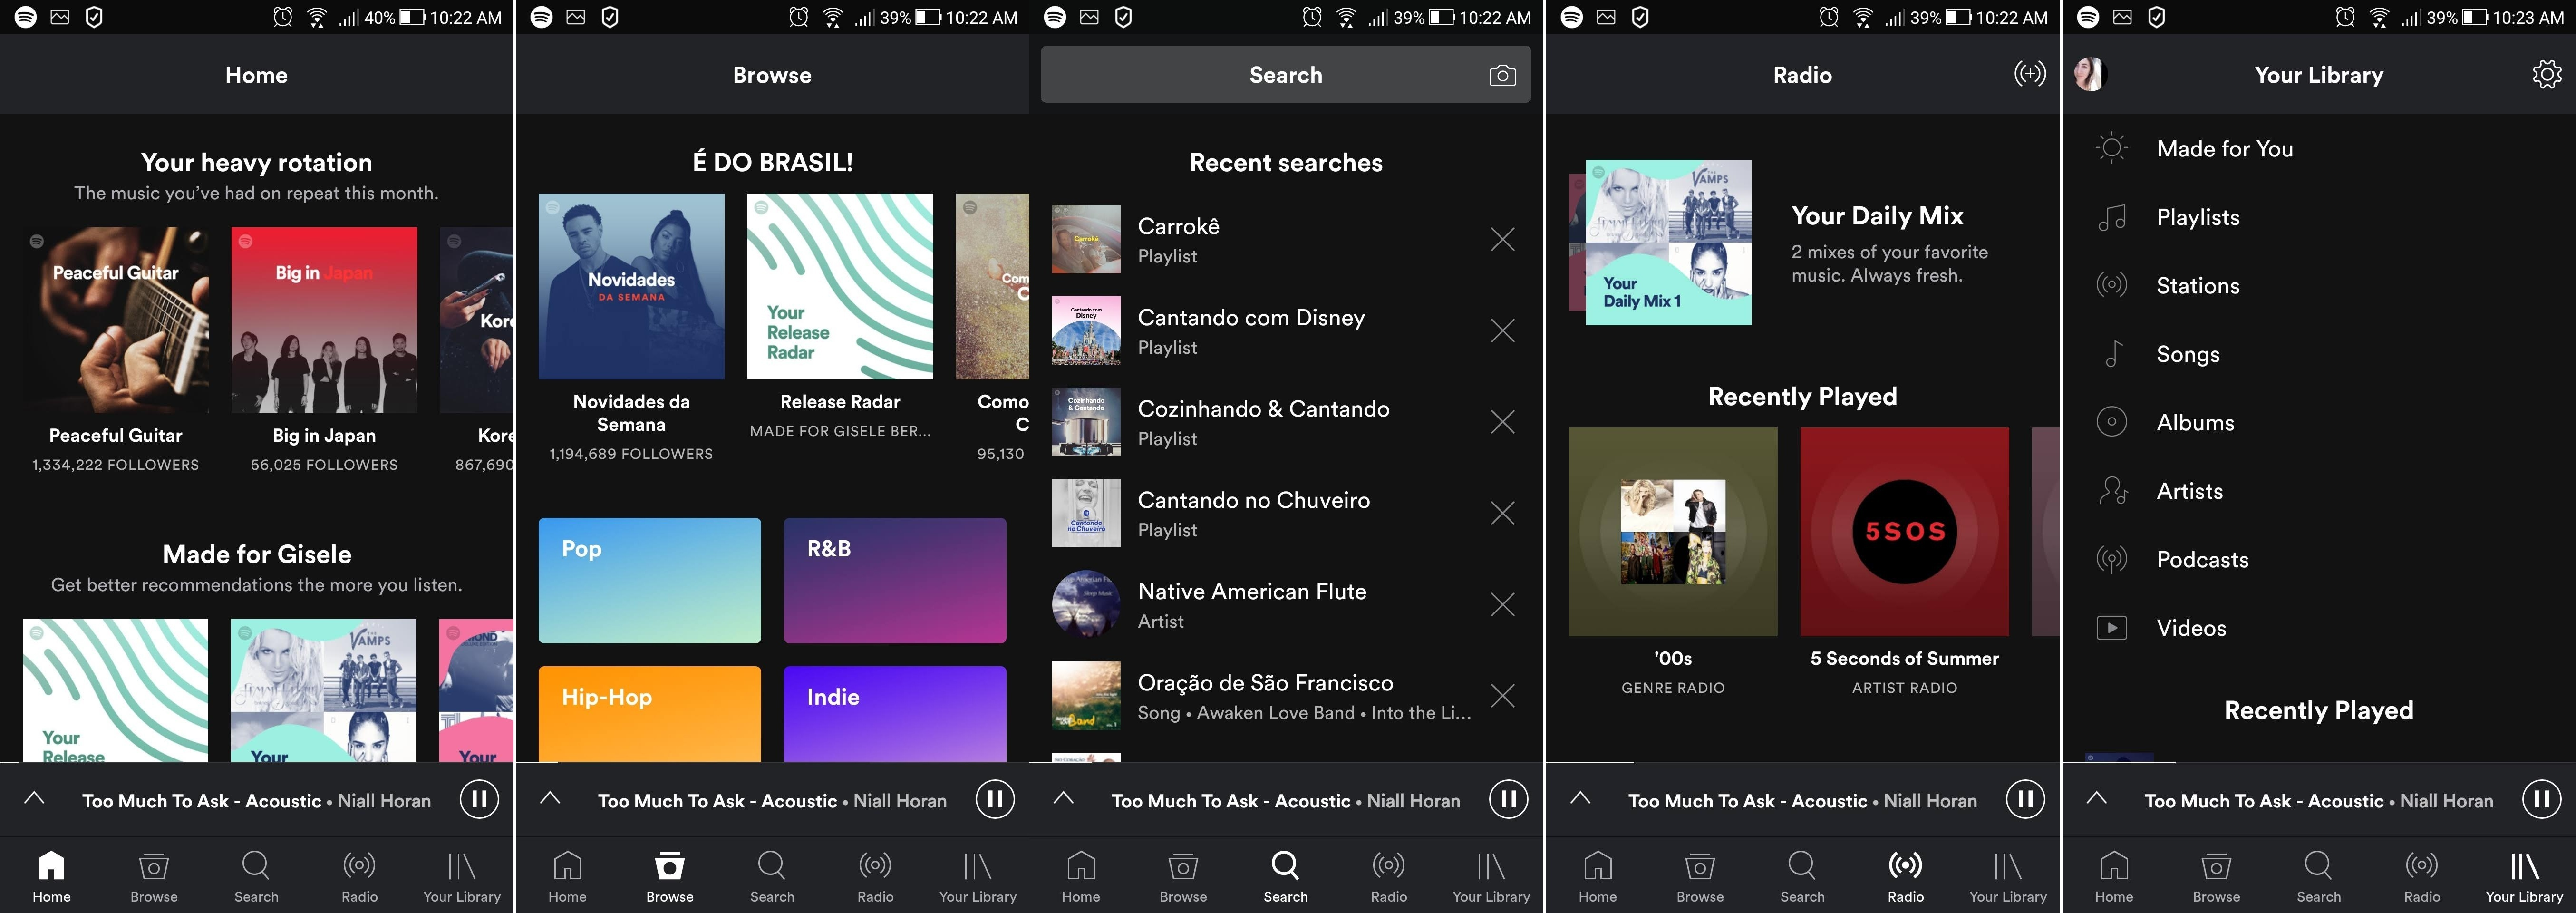
\includegraphics[scale=0.10]{figuras/spotify.jpg}
   \\Fonte: Elaborado pela autora
\end{figure}

Por sua vez, o SoundCloud (Ver Figura \ref{fig:soundcloud}) é similar ao Spotify, com a diferença de ser o único aplicativo comercial analisado que possui a possibilidade de inclusão de músicas criadas pelos usuários. Busca por música exclusiva por metadados, os componentes interativos são claramente distintos dos demais, com ícones compreensíveis, intuitivos, linguagem clara e de textos curtos. Funciona corretamente, sem apresentar problemas.

\begin{figure}[!htb]
   \centering
   \caption{SoundCloud}\label{fig:soundcloud} 
   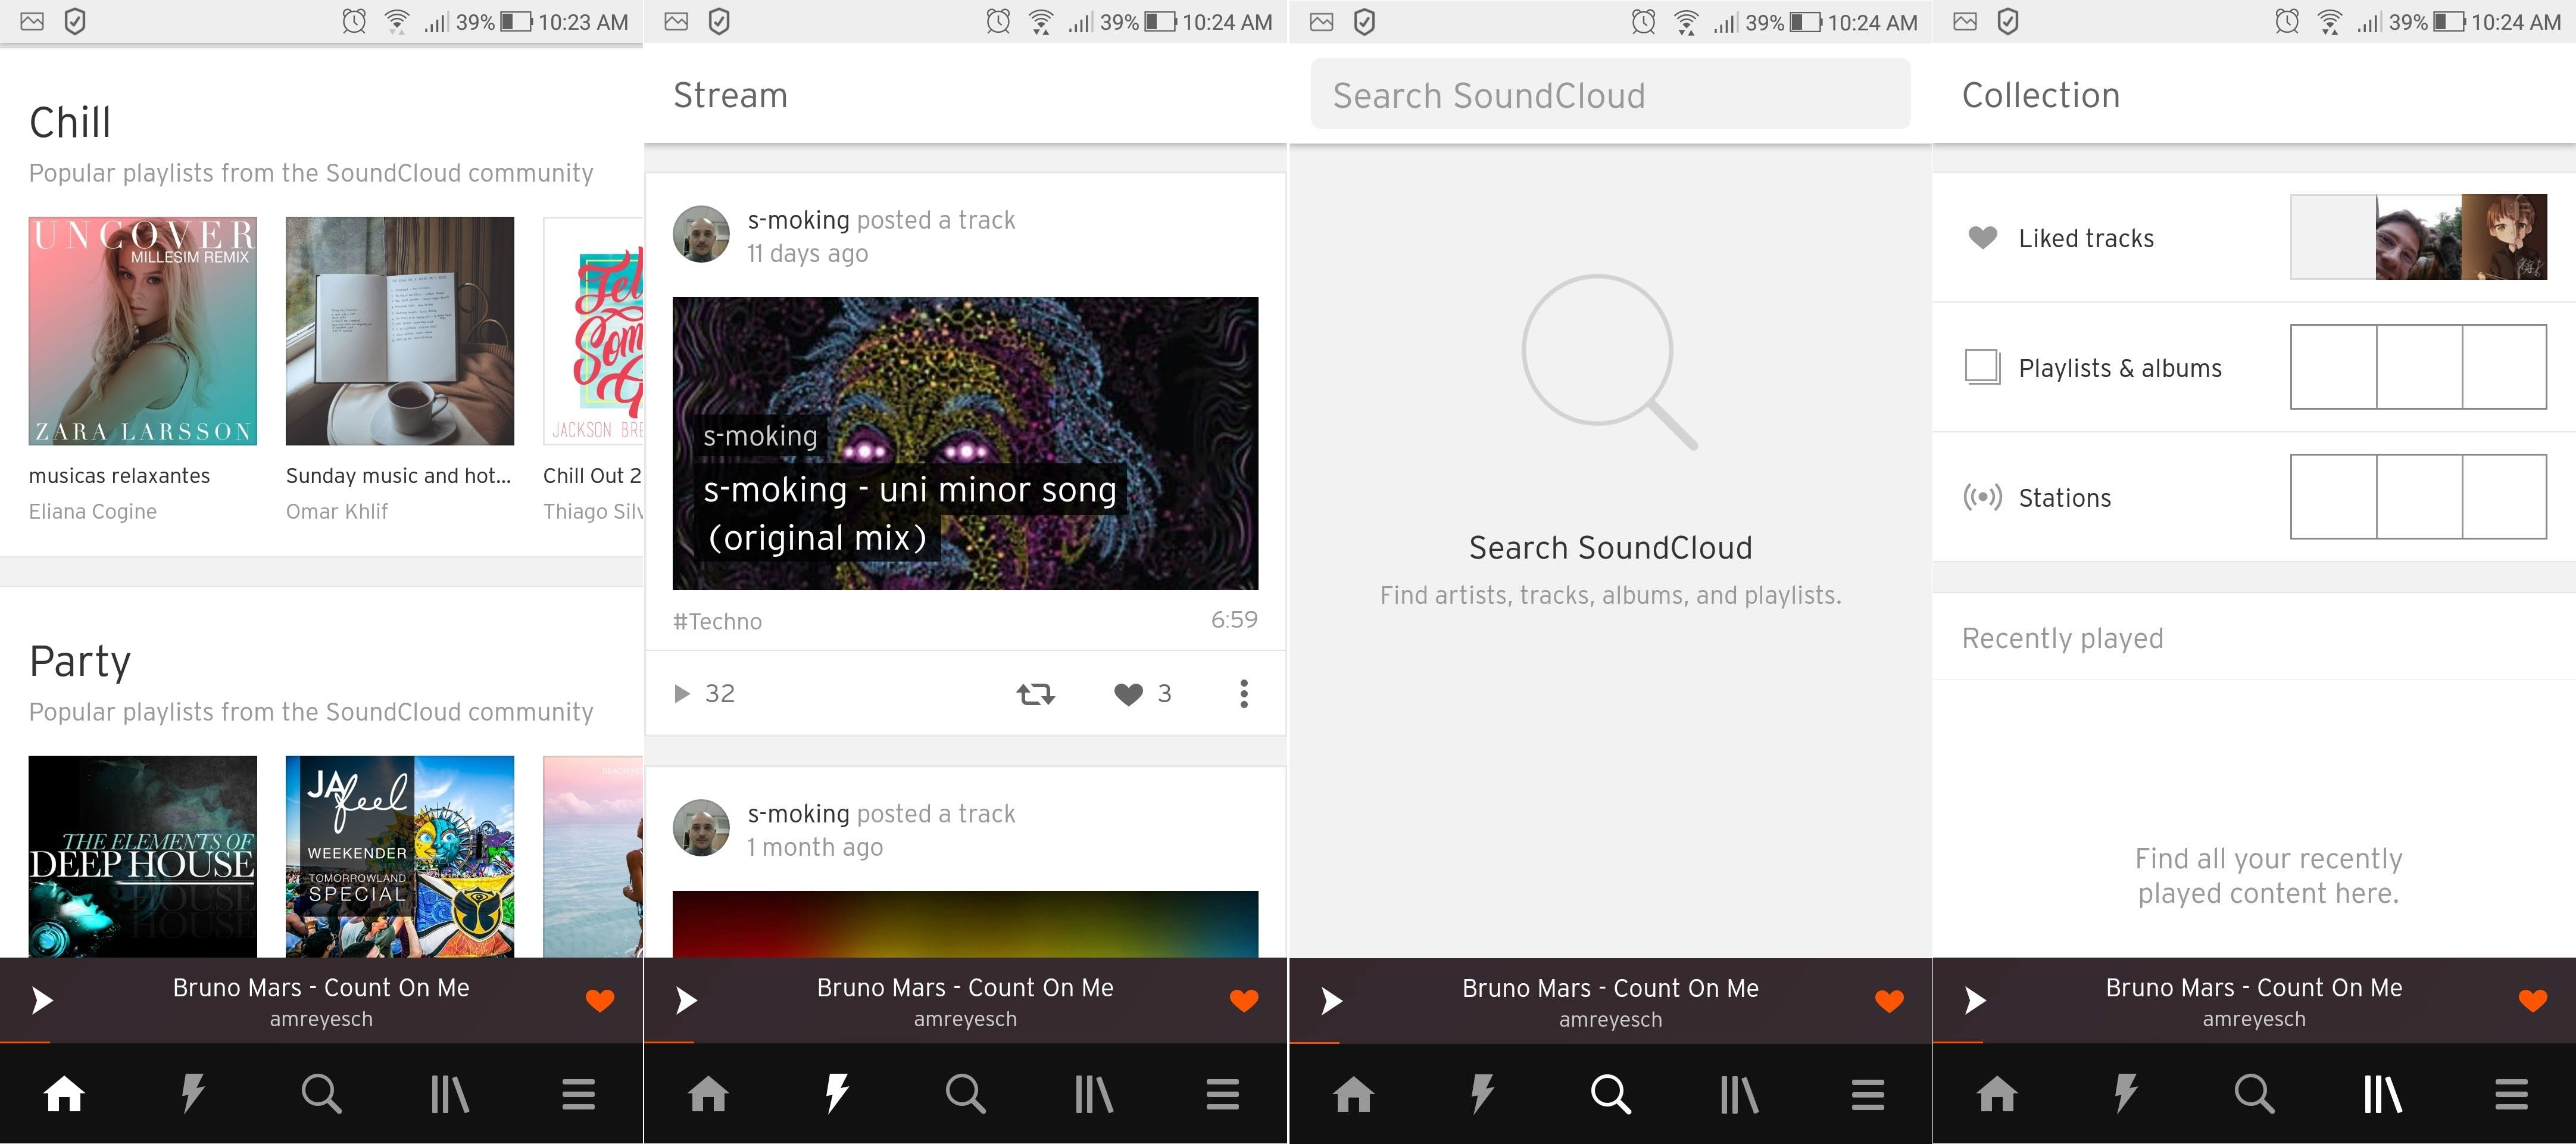
\includegraphics[scale=0.12]{figuras/soundcloud.jpg}
   \\Fonte: Elaborado pela autora
\end{figure}

O MusiXmatch (Ver Figura \ref{fig:musixmatch}) é simples, navegação intuitiva, sem muitas funcionalidades e de fácil execução, é um aplicativo que sincroniza letras de músicas, mas também oferece o reconhecimento delas. Os componentes interativos são claramente distintos dos demais, com ícones compreensíveis, intuitivos e possui uma linguagem clara e concisa. Funciona corretamente, sem apresentar problemas. O menu é esteticamente simples, claro e sem propagandas.

\begin{figure}[!htb]
   \centering
   \caption{MusiXmatch}\label{fig:musixmatch} 
   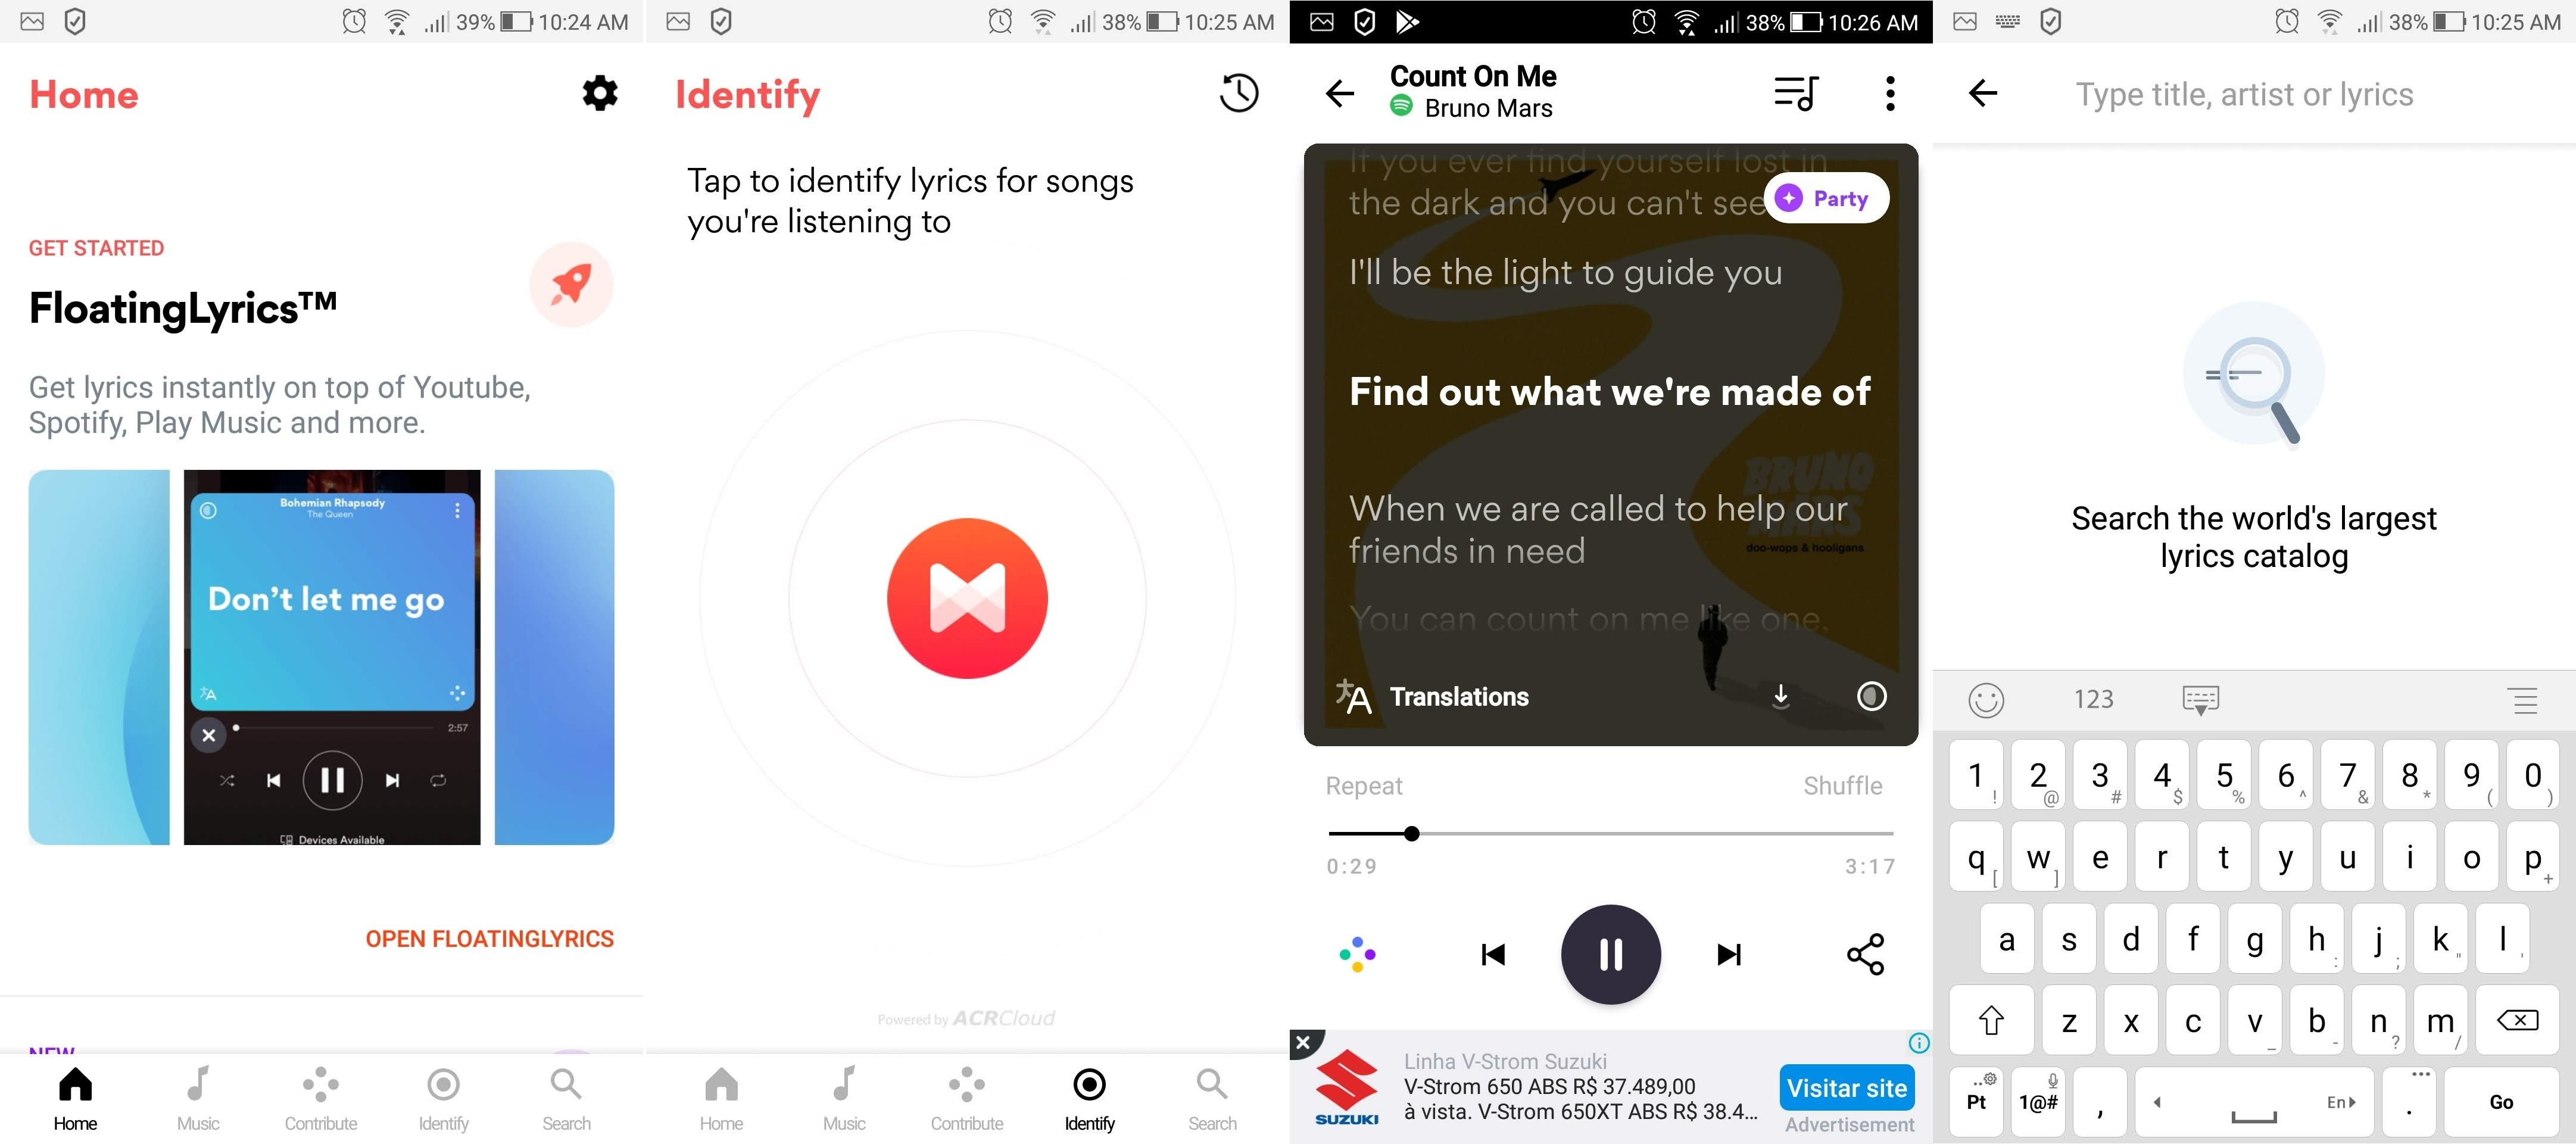
\includegraphics[scale=0.12]{figuras/musixmatch.jpg}
   \\Fonte: Elaborado pela autora
\end{figure}

O ACRCloud é um serviço de nuvem, com um enorme banco de dados musical. Além de oferecer o serviço de reconhecimento de músicas, possui também a possibilidade de fazer o reconhecimento de músicas pela web, como um teste do seu serviço. Navegação simples, os componentes interativos são claramente distintos dos demais, com ícones compreensíveis, intuitivos, linguagem clara e de textos curtos. Funciona corretamente, sem apresentar problemas.

\begin{figure}[!htb]
   \centering
   \caption{ACRCloud}\label{fig:acrcloud} 
   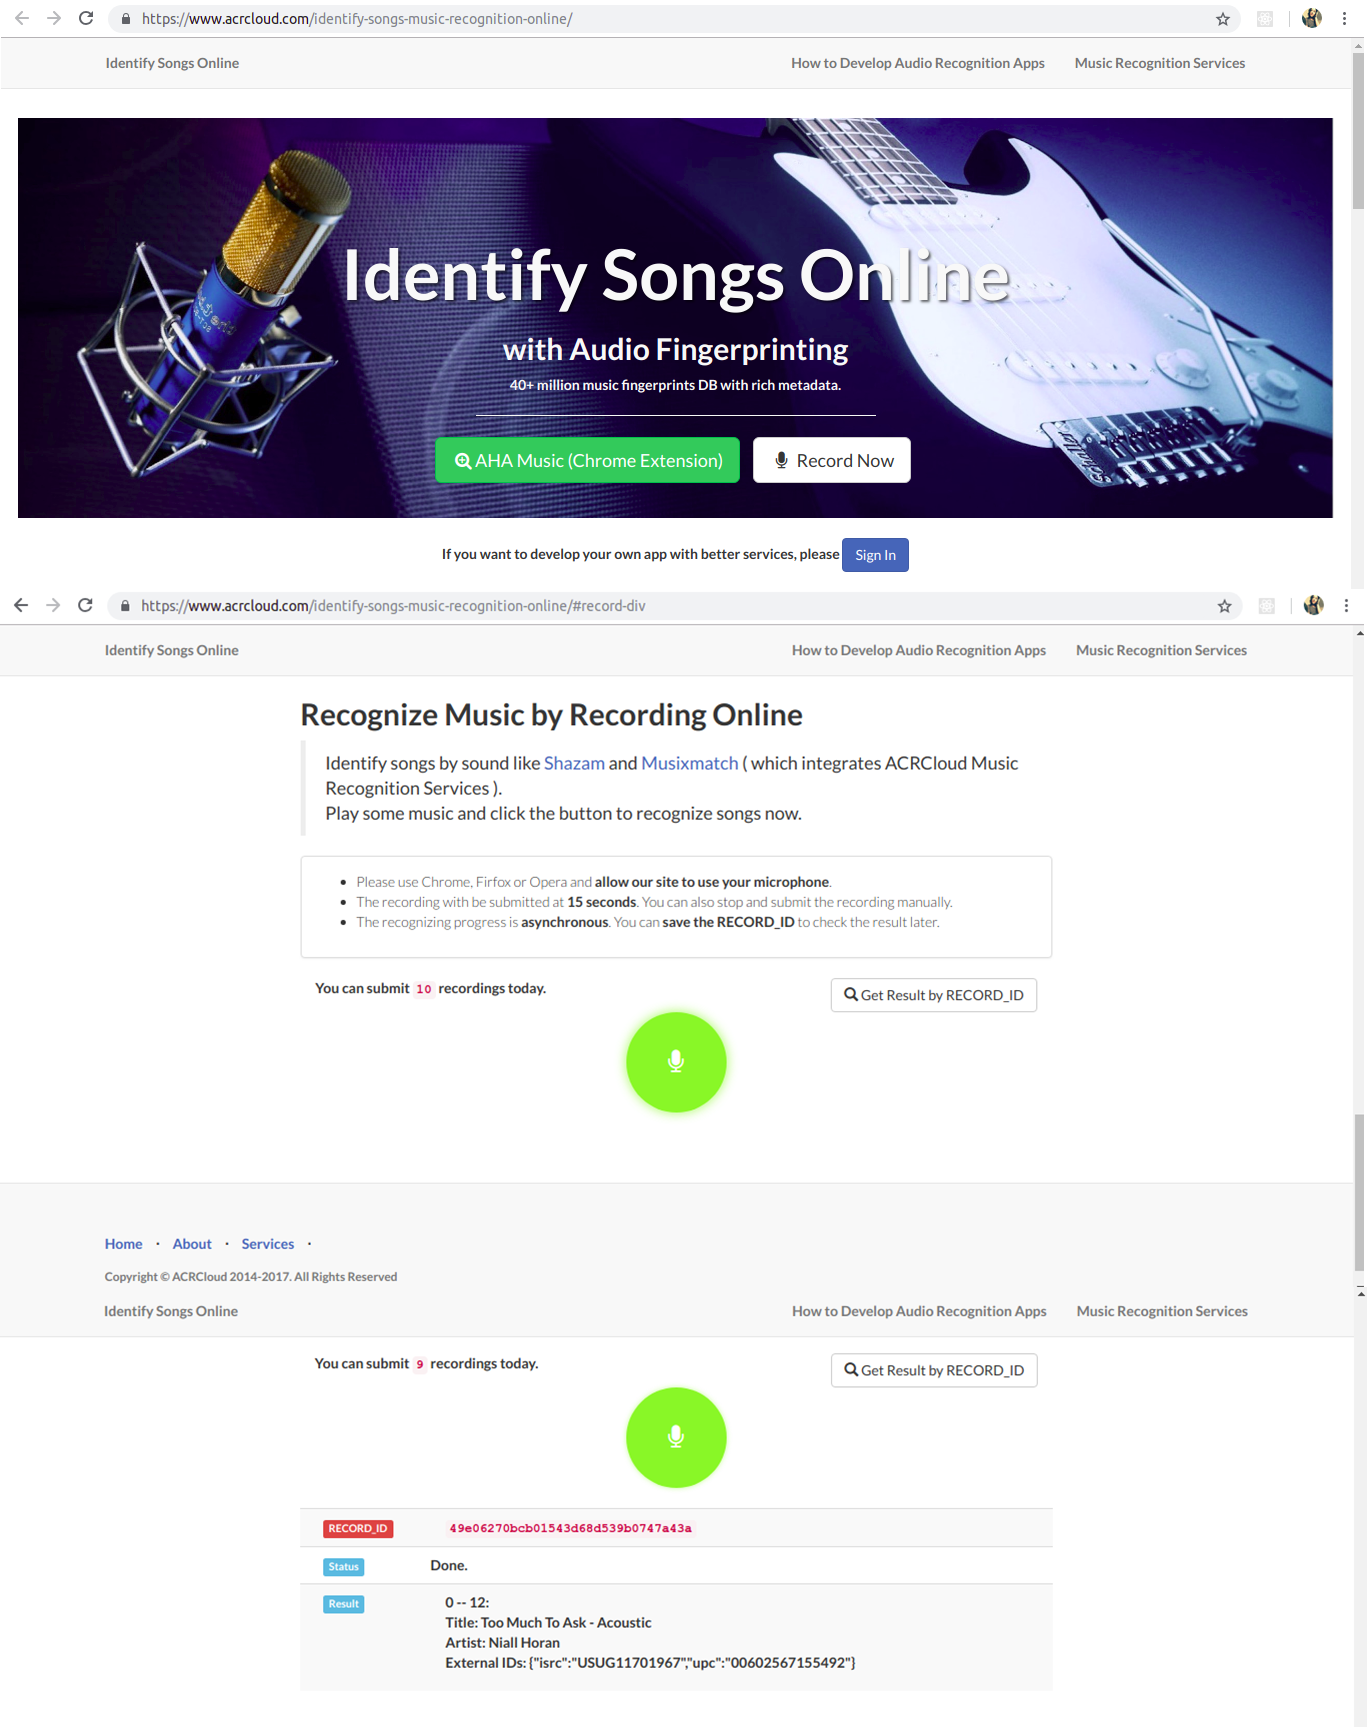
\includegraphics[scale=0.30]{figuras/acrcloud.png}
   \\Fonte: Elaborado pela autora
\end{figure}


%%%====== INICIO TABELA ======%%%
\begin{landscape}
\fontsize{8.5}{12}\selectfont
\tabcolsep=0.11cm
\begin{longtable}[c]{c|p{.09\textwidth}|p{.07\textwidth}|p{.065\textwidth}|p{.102\textwidth}|p{.10\textwidth}|p{.10\textwidth}|p{.10\textwidth}|p{.10\textwidth}|p{.09\textwidth}|p{.085\textwidth}|p{.10\textwidth}|p{.06\textwidth}|p{.06\textwidth}|p{.10\textwidth}|p{.07\textwidth}|p{.08\textwidth}|p{.06\textwidth}}
\caption{Comparação entre as Soluções, forma comercial e acadêmica}
\label{comparacaoCriterios}\\
\hline
\multicolumn{2}{c|}{\multirow{3}{*}{CRITÉRIOS}} & \multicolumn{16}{c}{SOLUÇÕES} \\ \cline{3-18} 
\multicolumn{2}{c|}{} & \multicolumn{9}{c|}{COMERCIAL} & \multicolumn{7}{c}{ACADÊMICO} \\ \cline{3-18} 
\multicolumn{2}{c|}{} & MusicID & Shazam & SoundHound & Deezer & Spotify & SoundCloud & Musixmatch & ACRCloud & Musipedia & MusicMiner & YALE & CLAM & MIRtoolbox & AMUSE & Java MIR & Tunebot \\ \hline
\endfirsthead
%
\multicolumn{18}{c}%
{{\bfseries \tablename\ \thetable\ continuação da página anterior}} \\
\hline
\multicolumn{2}{c|}{\multirow{3}{*}{CRITÉRIOS}} & \multicolumn{16}{c}{SOLUÇÕES} \\ \cline{3-18} 
\multicolumn{2}{c|}{} & \multicolumn{9}{c|}{COMERCIAL} & \multicolumn{7}{c}{ACADÊMICO} \\ \cline{3-18} 
\multicolumn{2}{c|}{} & MusicID & Shazam & SoundHound & Deezer & Spotify & SoundCloud & Musixmatch & ACRCloud & Musipedia & MusicMiner & YALE & CLAM & MIRtoolbox & AMUSE & Java MIR & Tunebot \\ \hline
\endhead
%
\multirow{3}{*}{\rotatebox[origin=c]{90}{Eficiência de desempenho}} & Comporta-mento em relação ao tempo & até 8s & até 8s & até 5s & até 10s & até 30s & até 30s & até 13s & até 5s & - & - & - & - & - & - & - & - \\ \cline{2-18} 
 & Utilização de recursos & FP & FP & IA & RPC e FP & RPC & RPC & RPC e FP & FP & Diversas & Diversas & - & SMS & Diversas & C & C e ML & QBH \\ \cline{2-18} 
 & Bitrate & até 128kbps & - & - & até 320kbps & até 320kbps & até 128kbps & - & - & - & - & - & - & - & - & - & - \\ \hline
\multirow{7}{*}{\rotatebox[origin=c]{90}{Adequação Funcional}} & Disponibi-lidade & iOS, Android & iOS, Android & iOS, Android & iOS, Android, Windows, Web, Roku TV & Linux, Windows, OS X, iOS, Android, Web & iOS, Android & iOS, Android & Web & Web & Linux, Mac OSX, Windows & - & Linux, Mac OSX, Windows & Linux, Mac OSX, Windows & - & Linux, Mac OSX, Windows & iOS \\ \cline{2-18} 
 & Modelo de desenvolvimento & F & F & F & F & F & F & F & F & A & A & - & A & A & A & F & F \\ \cline{2-18} 
 & Integrações & não & Spotify, Google Play Music, Apple Music & Twitter, Youtube, Spotify & não & não & não & Spotify, Google Play Music, Deezer, Youtube & ISRC, UPC, Spotify, Deezer, Youtube, LyricFind, Music Story e SyncPower & não & não & Music-Miner, AMU-SE & não & não & MIRtoolbox & não & Karaoke Callout \\ \cline{2-18} 
 & Acessibi-lidade & On & On & On & On/Off & On/Off & On & On & On & On & Off & - & Off & Off & Off & Off & On?/Off \\ \cline{2-18} 
 & Busca de dados & aprox. & exato & aprox. & exato & exato & exato & aprox. & aprox. & aprox. & aprox. & aprox. & aprox. & aprox. & aprox. & aprox. & aprox. \\ \cline{2-18} 
 & Inclusão de dados & não & não & não & não & não & sim & não & sim & sim & sim & sim & sim & sim & sim & sim & sim \\ \cline{2-18} 
 & Modelo de pagamento & G & G & F & F & F & F & F & P & G & G & - & G & G & G & G & G \\ \hline
\multirow{5}{*}{\rotatebox[origin=c]{90}{Usabilidade}} & Visibilida-de do status do sistema & sim & sim & sim & sim & sim & sim & sim & sim & sim & - & - & - & - & - & - & - \\ \cline{2-18} 
 & Prevenção de erros & sim & sim & sim & sim & sim & sim & sim & sim & não & - & - & - & - & - & - & - \\ \cline{2-18} 
 & Flexibili-dade e eficiência de uso & sim & sim & sim & sim & sim & sim & sim & sim & sim & - & - & - & - & - & - & - \\ \cline{2-18} 
 & Estética e Design minimalista & sim & sim & sim & sim & sim & sim & sim & sim & não & - & - & - & - & - & - & - \\ \cline{2-18} 
 & Pouca interação homem / dispositivo & sim & sim & sim & sim & sim & sim & sim & sim & sim & - & - & - & - & - & - & - \\ \hline
\caption*{Legenda: FP - FingerPrint; IA - Inteligência Artificial; RPC - Recuperação por Conteúdo; SMS - Spectral Modeling Synthesis; C - Classificação; QBH - Query by Humming; A - Aberto; F - Fechado; G - Gratuito; F - Freemium; P - Premium}
\end{longtable}
\end{landscape}
%%%====== FIM TABELA ======%%%

\section{Resultados}
Resultados da comparação e análise das soluções propostas.
